\subsection{User View}

%For the main pages put a mockup and describe it in detail.

The home page, figure \ref{fig:user-home}, allows the user to browse through all the available restaurants where it is also possible to search for a restaurant by name (part of the name) and by cuisine type. Once clicked on a restaurant from the list, a new page is shown with all the dishes a restaurant can sell (figure  \ref{fig:user-MenuPage}). Here we can also notice how the side panel changes if the user has already logged in or not. If a guest user tries to add an item to the cart a login popup will show (figure \ref{fig:user-login}). In figure  \ref{fig:user-registration} and in figure  \ref{fig:user-update} we can see respectively the user registration and the user update forms.

\begin{center}
	\frame{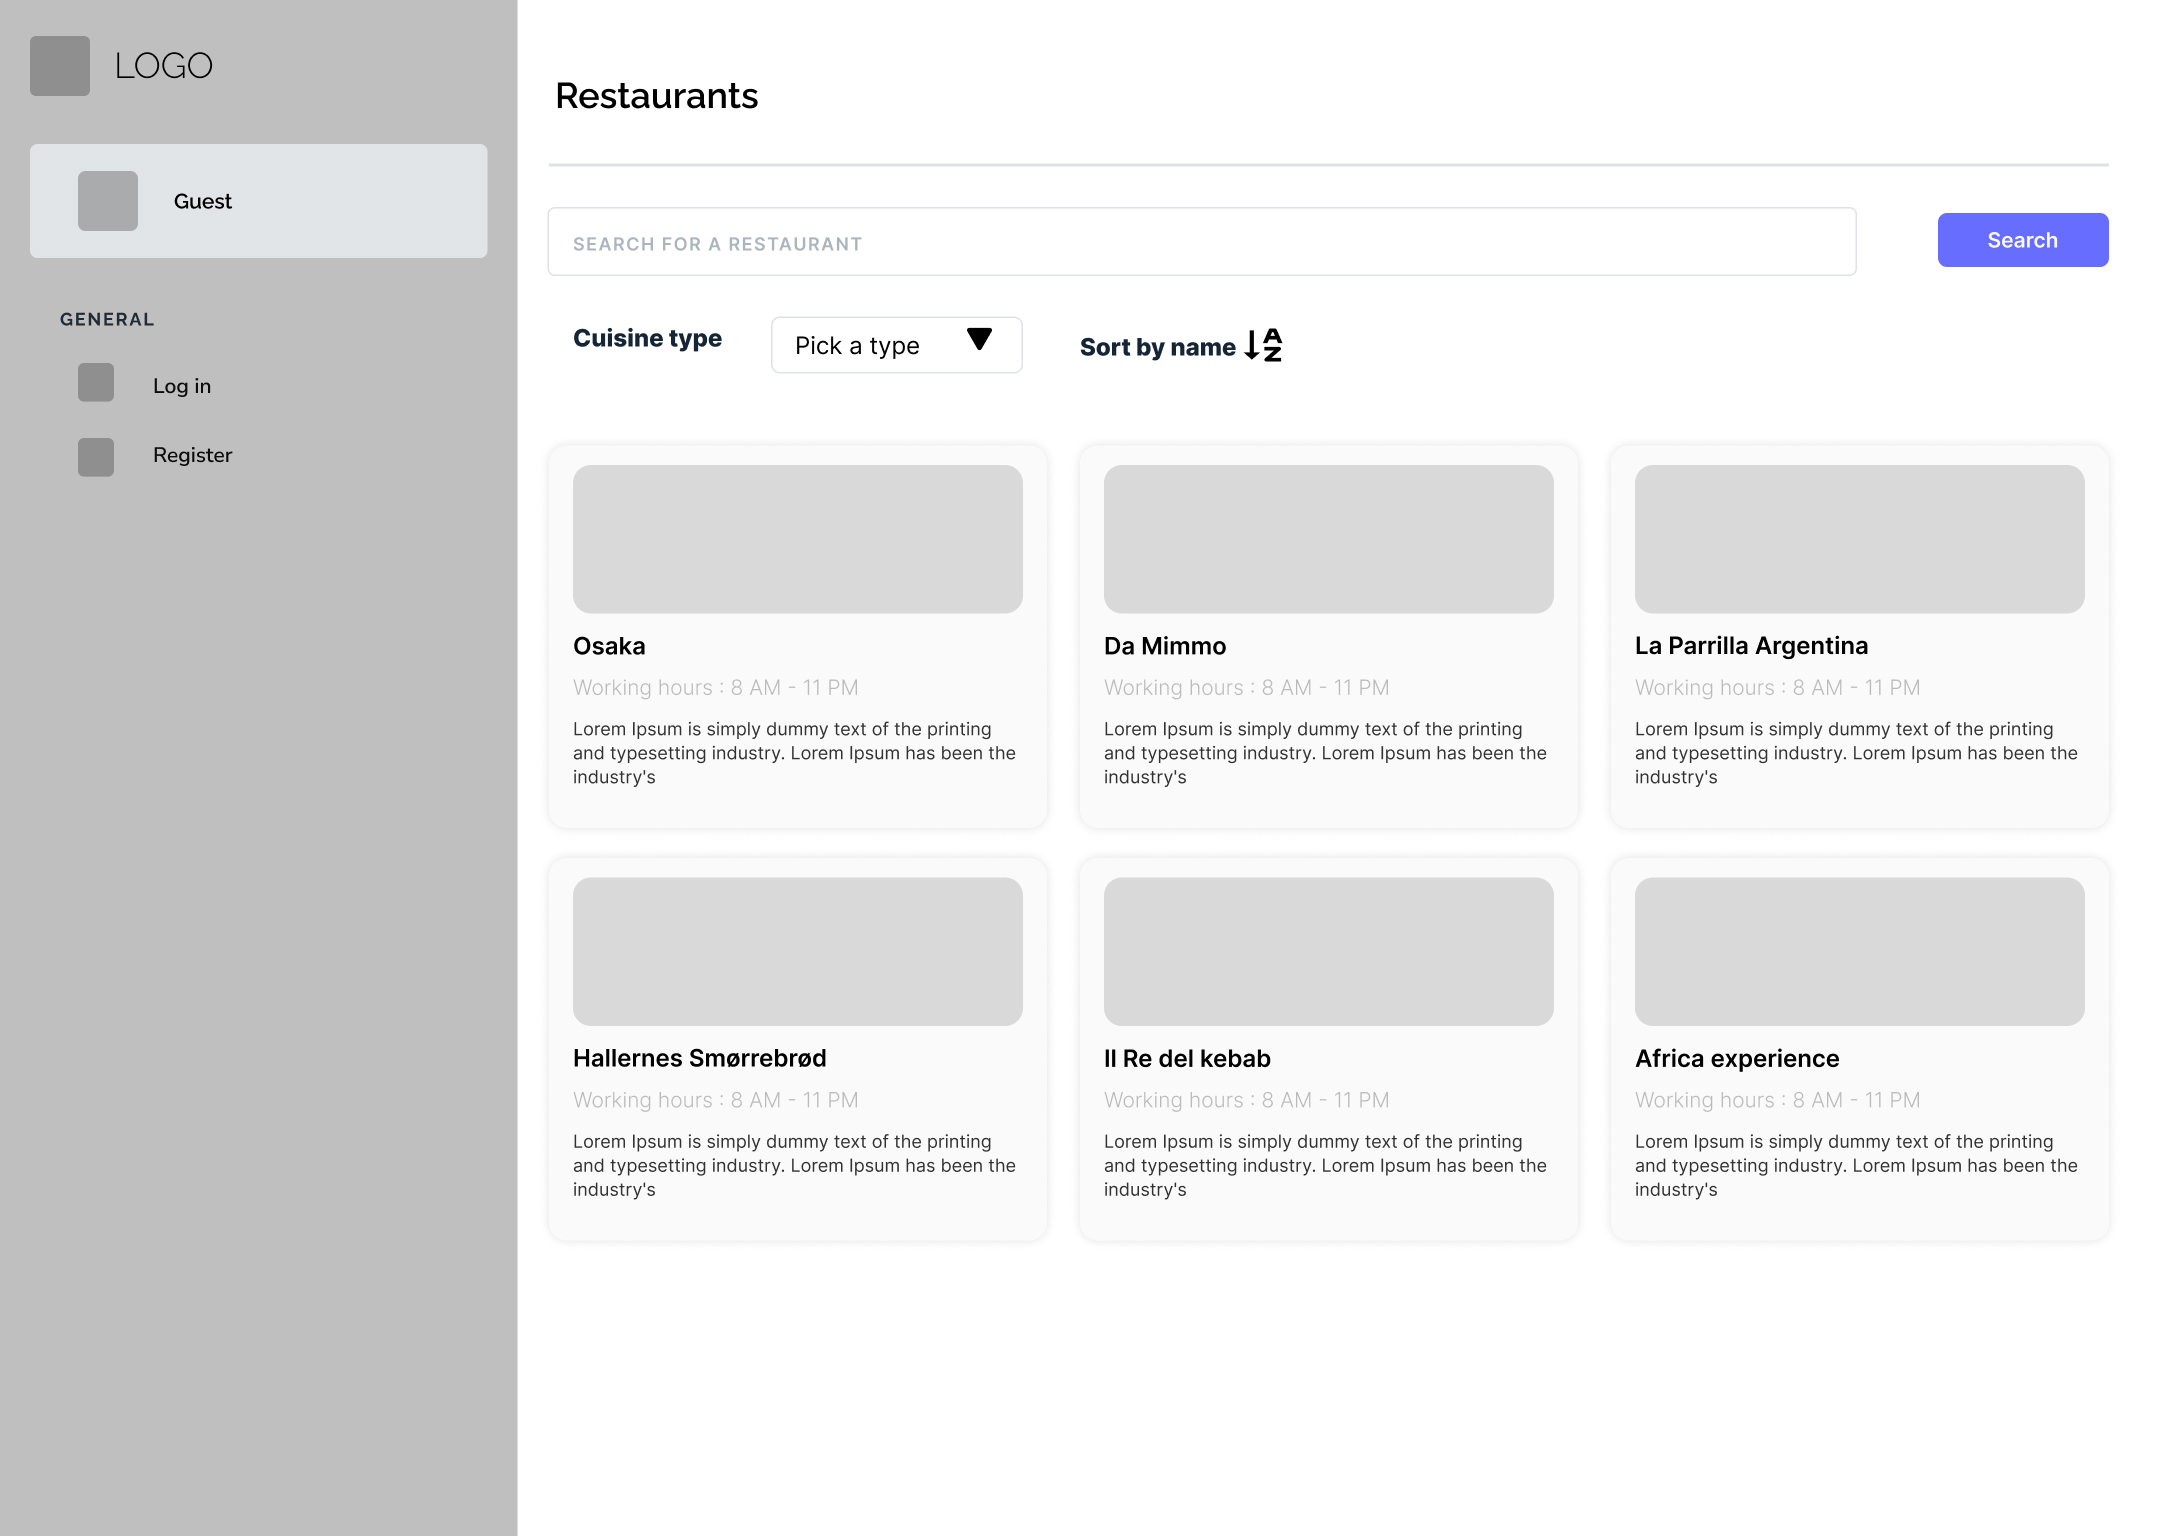
\includegraphics[width=.8\textwidth]{resources/mockup/user/Home_logged-out.jpg}}
	\captionof{figure}{Home Page.}
	\label{fig:user-home}
\end{center}


\begin{center}
	\frame{\includegraphics[width=.8\textwidth]{resources/mockup/user/menu.jpg}}
	\captionof{figure}{Restaurant's menu page.}
	\label{fig:user-MenuPage}    
\end{center}


\begin{center}
	\frame{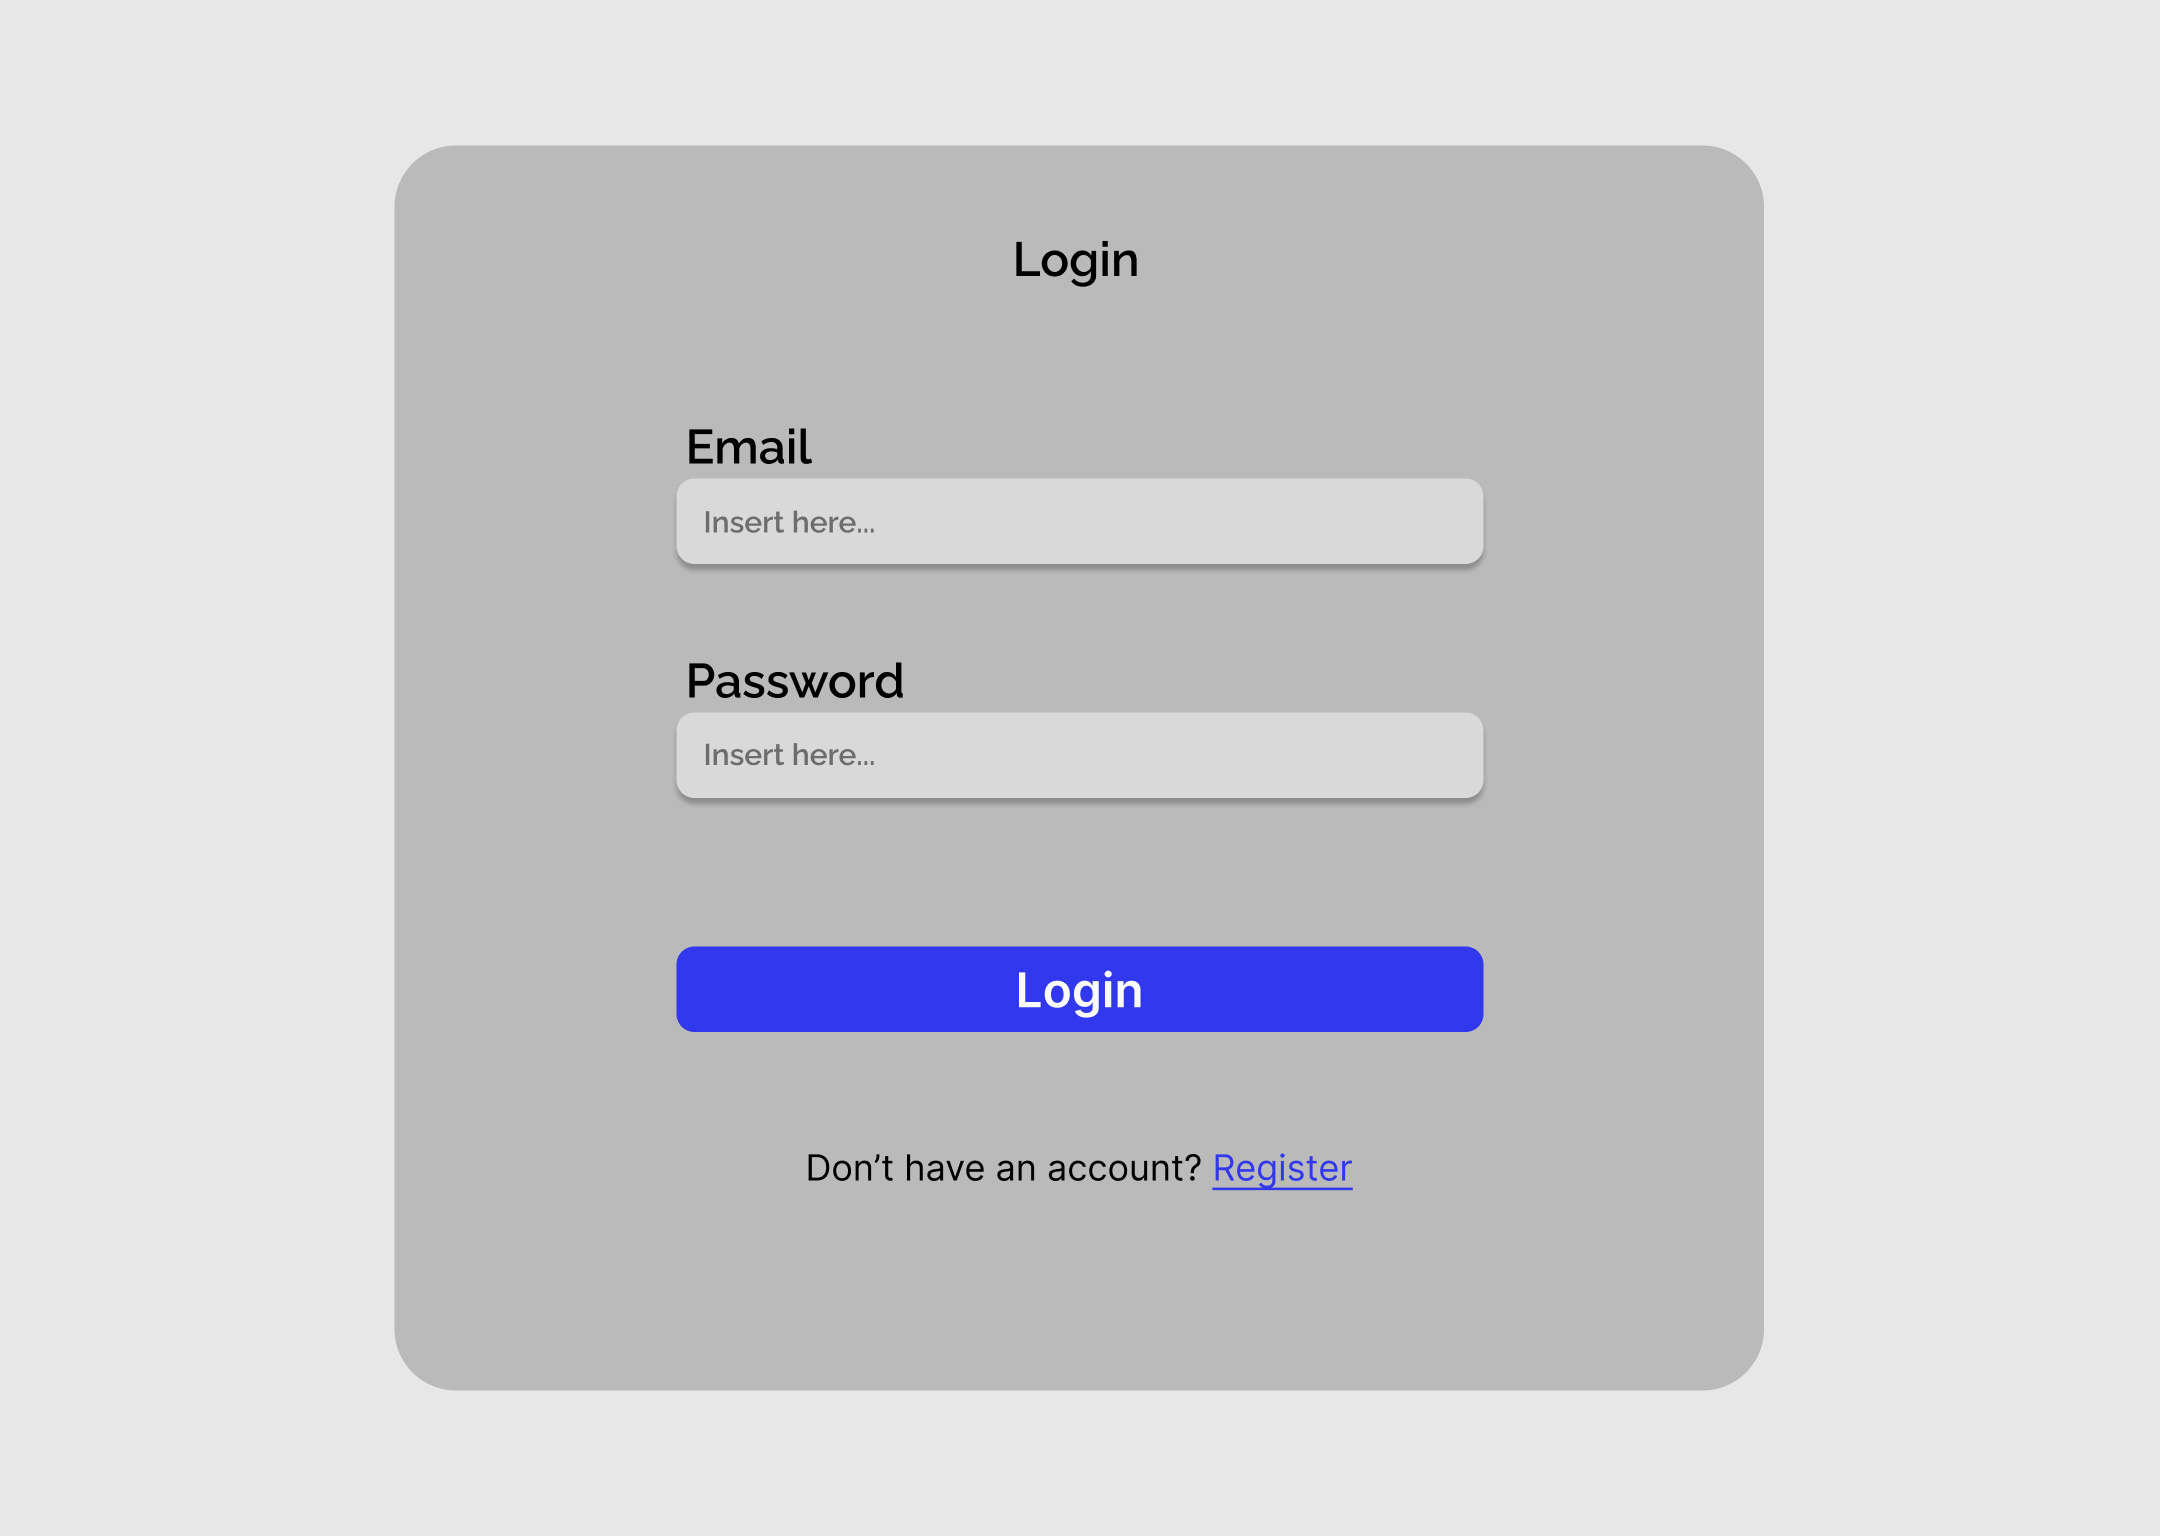
\includegraphics[width=.8\textwidth]{resources/mockup/user/Login.jpg}}
	\captionof{figure}{User login page}
	\label{fig:user-login}    
\end{center}


\begin{center}
	\frame{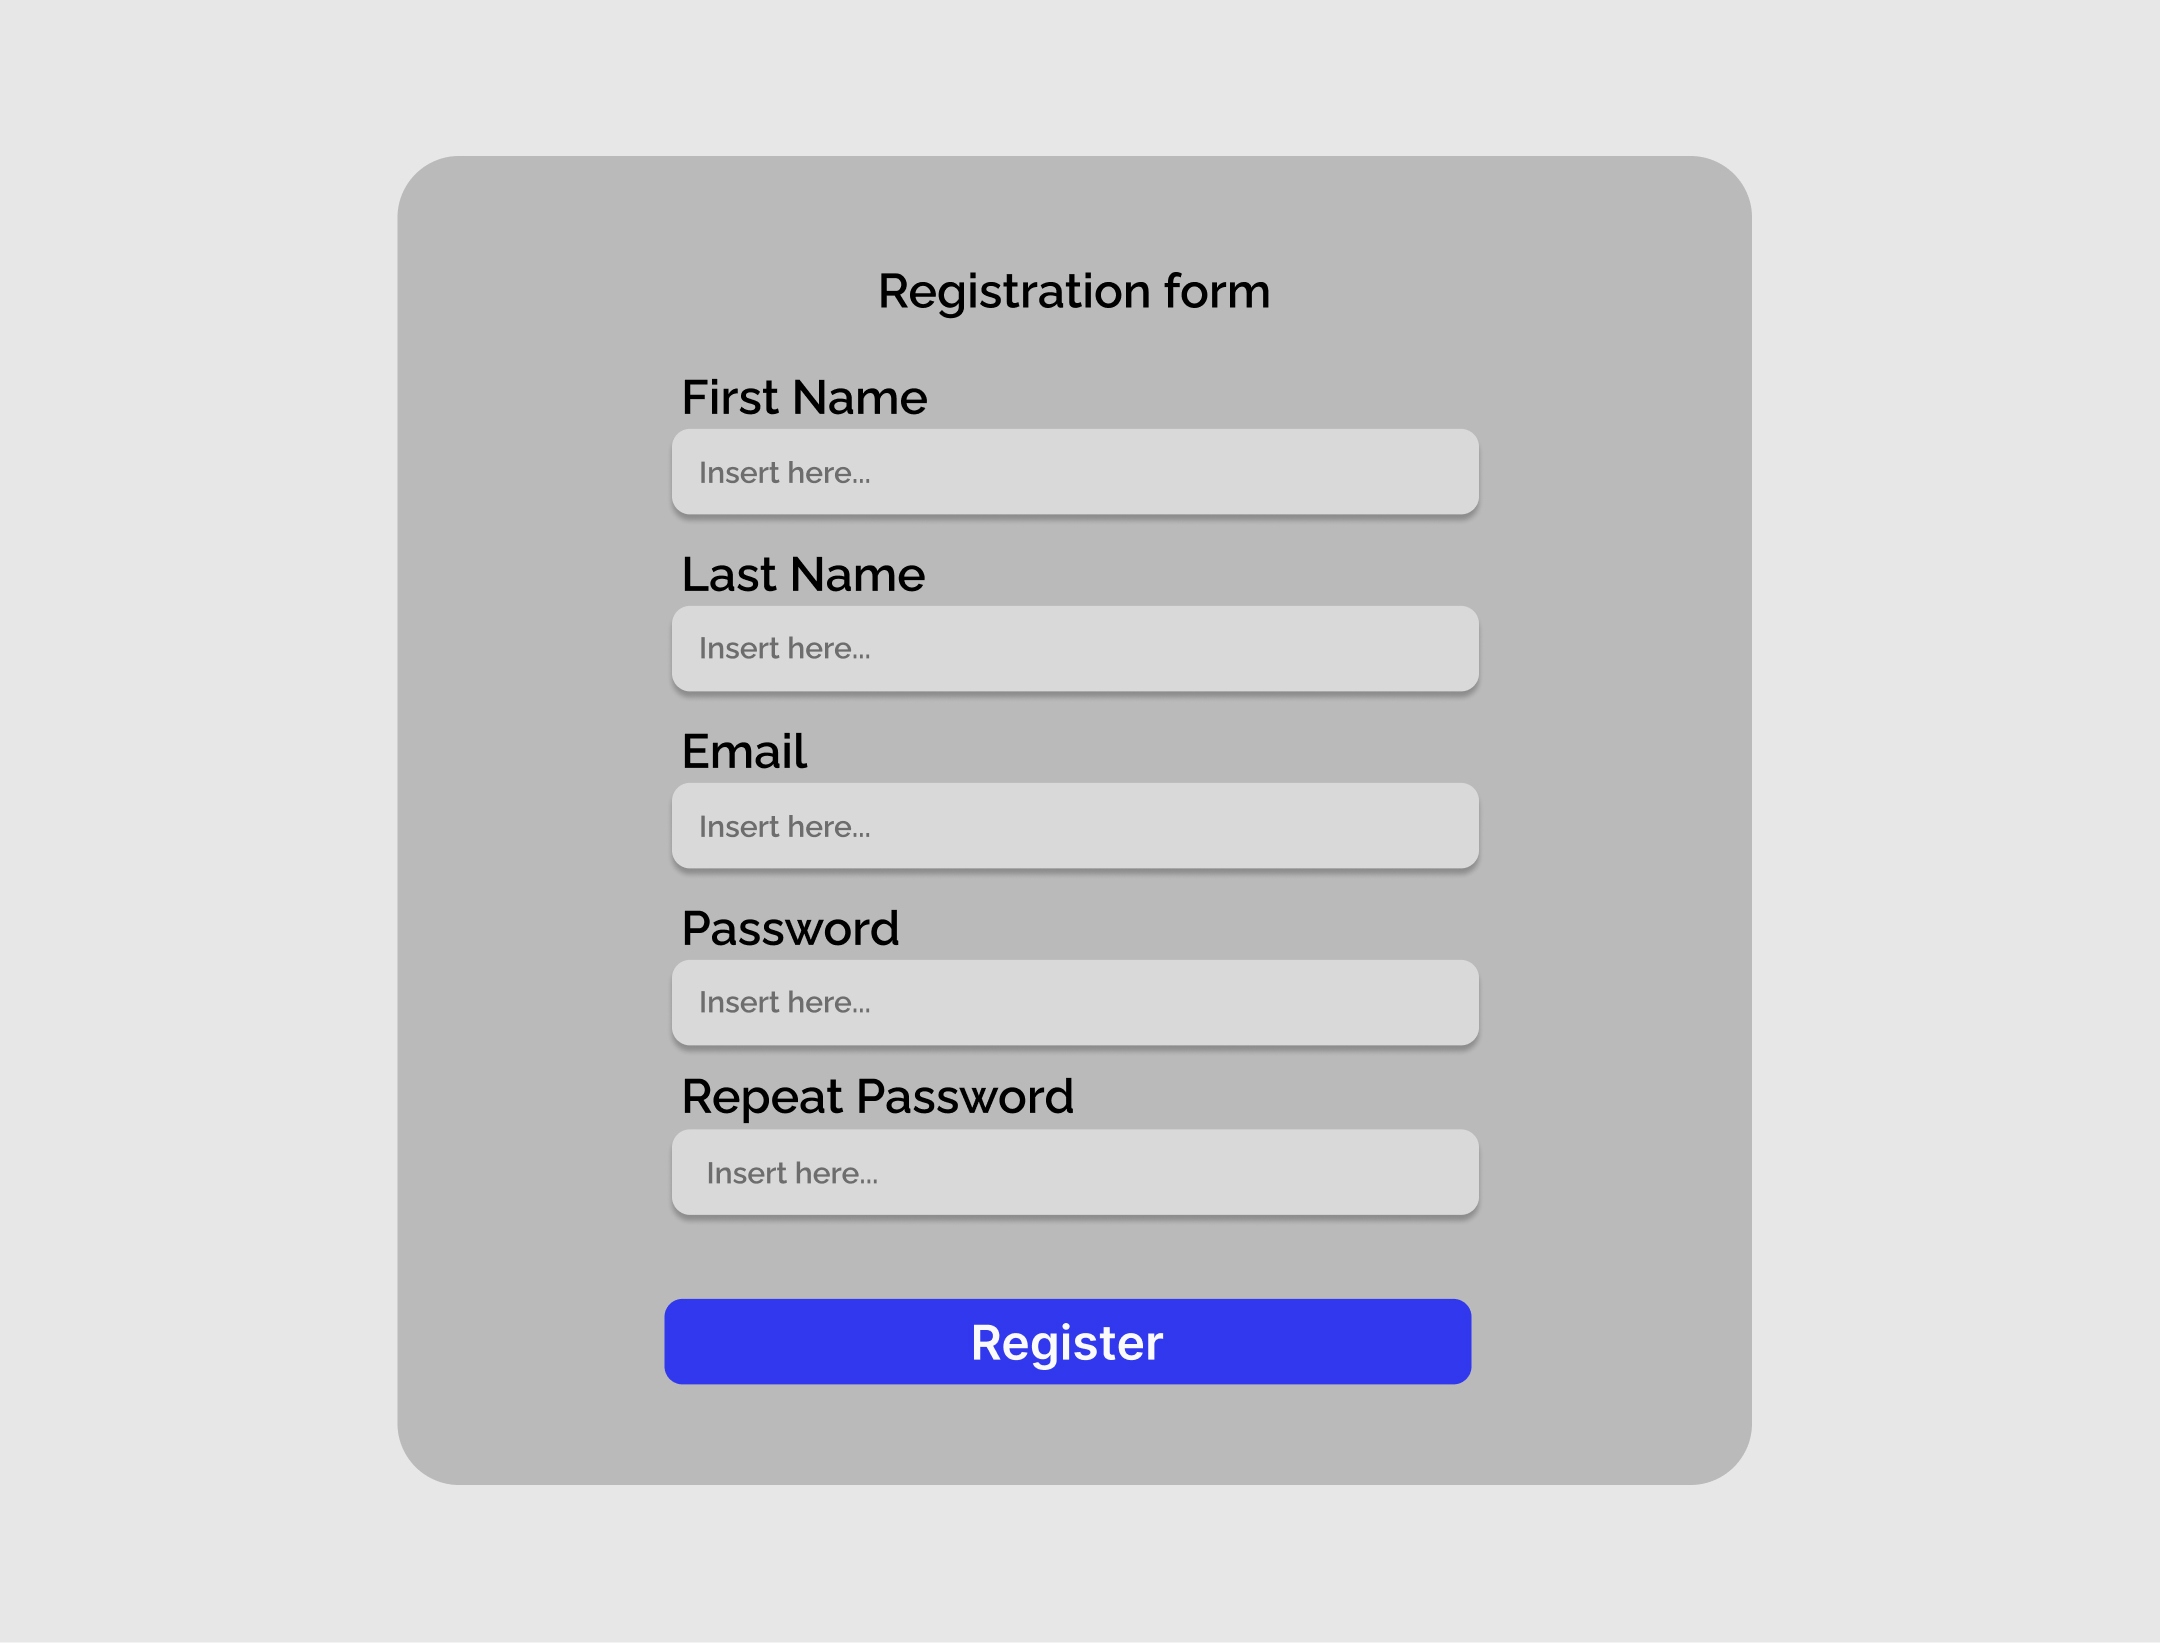
\includegraphics[width=.75\textwidth]{resources/mockup/user/Register.jpg}}
	\captionof{figure}{User registration page.}
	\label{fig:user-registration}    
\end{center}

\begin{center}
	\frame{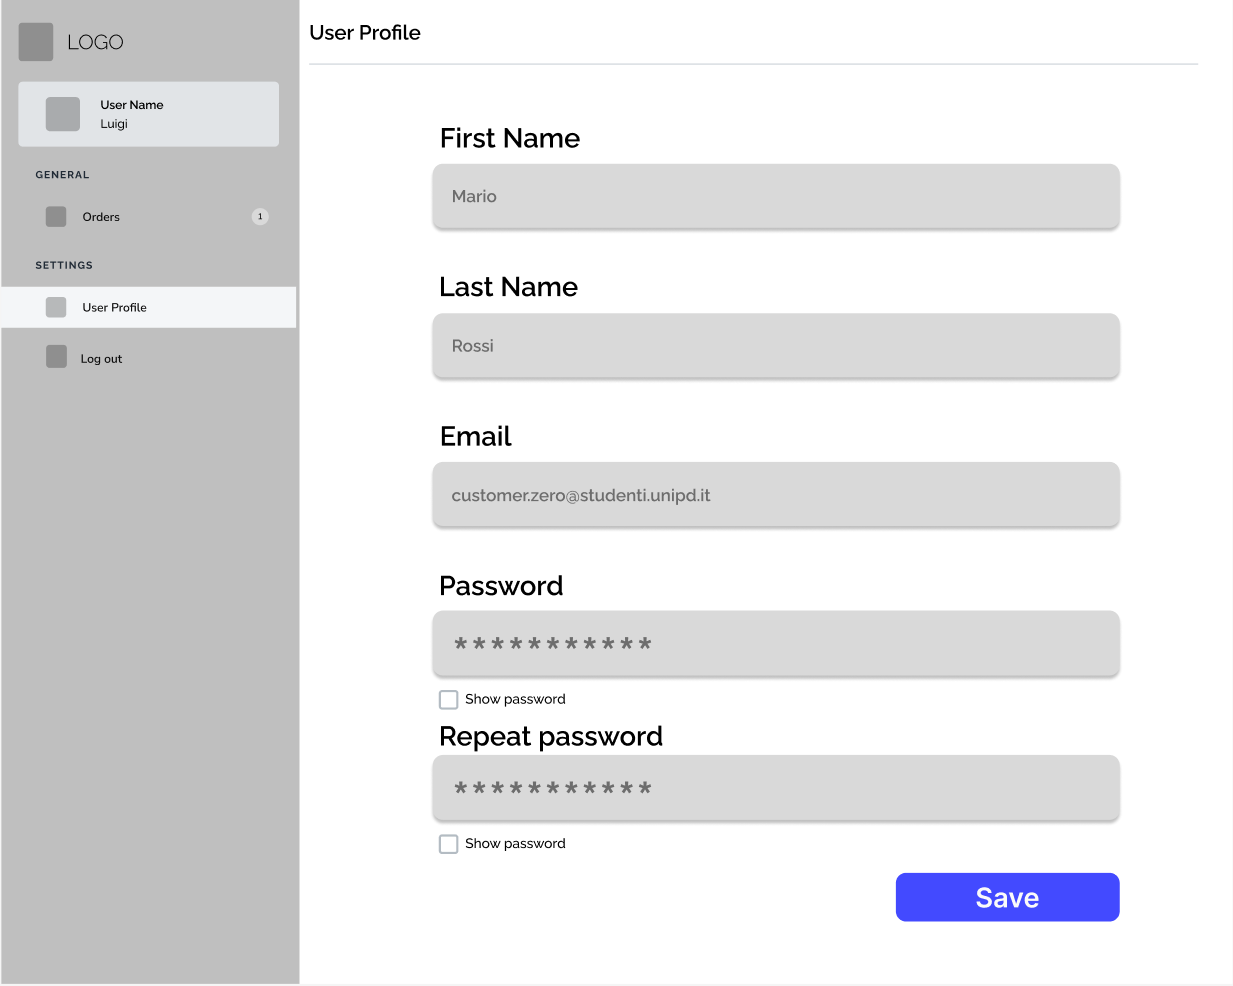
\includegraphics[width=.75\textwidth]{resources/mockup/user/UpdateUserProfile.png}}
	\captionof{figure}{Update user profile page.}
	\label{fig:user-update}    
\end{center}

